\chapter{\rtd\ and \ee\ tutorial for \avr5}

This small tutorial describes a set of steps needed to compile a
simple application that shows the main features of \ee\ and \rtd\ for
the \avr\ platform.

This tutorial has been tested on a STK50X board produced by Atmel
and on a Crossbow Mib520 board.




\chapter{Installing \ee\ and \rtd\ on Microsoft Windows}
\label{cha:installing}

This chapter will guide the developer to the installation procedure of
\ee\ and \rtd\ for the \avr\ platform.

\begin{warning}
The Cygwin install pathname, the \ee\ install pathname, and the 
pathname of \rtd\ workspaces where the user projects reside, MUST NOT 
contain any blank space, otherwise \ee\ may not work properly.

E.g., \file{C:\\MyApplications\\Evidence\\} and 
\file{C:\\MyApplications\\Cygwin\\} are acceptable, while 
\file{C:\\My Applications\\Evidence\\} or 
\file{C:\\My Applications\\Cygwin\\} MUST be avoided.

This is a known issue that will soon be fixed.
\end{warning}

The installation of \ee\ and \rtd\ is composed by the following
packages:
\begin{itemize}
\item The Eclipse development environment, which is used by \rtd\ to
  provide the basic development environment for \ee\ applications.
\item The Eclipse environment is based on the Java platform, so that
  a working Java Runtime Environment must be present for using \rtd.
\item The \rtd\ plugins, which provide the code generation for \ee\
  and \ee\ for Eclipse.
\item The \ee\ source code.
\item A subset of the Cygwin environment \cite{cygwin}, including
  a set of utilities like \file{make}, \file{gawk}, and few others, which
  are used during the compilation process of an \ee\ application.
\item A set of examples for the \avr\ Platform, which can be used to
  compile a first set of running examples for the Atmel STK50X board, the
  Crossbow MIB5X0 board. 
  These applications are organized in ``templates'', available at project 
  creation.
\end{itemize}

To install the software, execute the following steps:

\begin{enumerate}

\item Install your favourite Java runtime environment, which is needed
  to run \rtd; in fact, \rtd\ is a plugin of the Eclipse editor, which
  requires Java to be executed.

\item Install the AVR-Gcc Compiler, available from the WinAVR sourceforge.net 
  project at the website \url{http://winavr.sourceforge.net/}.  
  Even in this case, you can use the default install directory. 
  When it is asked to change the default environment, please do accept.

\item Run the \ee\ and \rtd\ installer.

\item The installer will prompt a list of packages which can be
  installed. Select all the packages you wish to install and
  continue the installation procedure (see Figure \ref{fig:installer-options}).
%
\begin{figure}[htb]
\begin{center}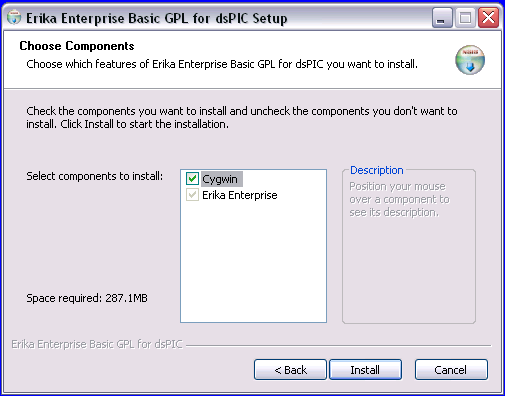
\includegraphics[
  width=8cm, bb=0 0 505 396]{images/installer_options.png}\end{center}
\caption{This screenshot shows the dialog box with the available install packages.}
\label{fig:installer-options}
\end{figure}

\item At this point, please check the {\em first} line of the file
  \file{evidencedir\\bin\\mymake_cygwin.bat} (where \file{evidencedir}
  is the directory you chose during the installation). For example,
  if Cygwin is installed inside \file{C:\\cygwin}, then the first line
  of the file should look like the following one:
\begin{lstlisting}
@set EE_BASH_PATH=C:\cygwin\bin\bash
\end{lstlisting}
  ...that is, the line contains the correct path to the
  \file{bash.exe} file in your Cygwin installation. If you accepted
  the default settings, the correct pathname should be
  \file{C:\\cygwin\\bin\\bash} as specified in the example before.
  \begin{note}
    We ask to perform this check because it seems that on some Windows
    machines the Cygwin installer does not correctly set the registry
    keys used by the \ee\ installer.
  \end{note}

\item If you are going to use the Atmel stk50x or the Crossbow Mib5x0
  boards, you can use the UISP programmer to program the \avr\
  microcontroller. To Install the UISP software, which is an AVR
  In-system Programmer using the USB connection provided by the boards
  cited above, please follow the instructions below:
  \begin{itemize}
  \item If not installed, run the Cygwin setup from
    \url{http://www.cygwin.com} to install the following Cygwin
    packages: gcc.
 
 \item Install the UISP - AVR in-System Programmer, available  at the 
    website \url{http://www.nongnu.org/uisp/}.  
\end{itemize}

\end{enumerate}

The rest of this tutorial supposes that the AVR-Gcc Compiler and binutils is
installed within the \file{C:\\WinAVR-20071221\\bin} directory.
Please note that these values may be different from the settings you have 
chosen on your machine.

\chapter{First \rtd\ startup and configuration}

After all the required packages have been installed, you are ready to
start \rtd\ for the first time.

Please follow the next steps:

\begin{enumerate}
\item As the first step, run the Eclipse IDE from the Evidence menu
  inside the Start menu of your Windows machine, choosing 
  \file{Start/Programs/Evidence/RT-Druid}.
  
\item A dialog box will appear, asking to choose the right
  workspace (see Figure \ref{fig:select-workspace}). 
  Leave the default workpackage directory
  as it is, and proceed by pressing ``OK''.
%
\begin{figure}[htb]
\begin{center}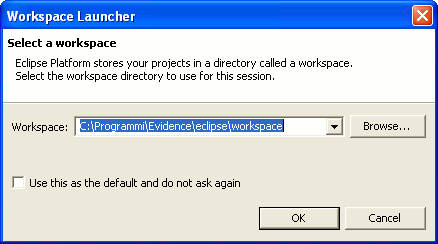
\includegraphics[
  width=8cm, bb=0 0 438 244]{images/select_workspace.png}\end{center}
\caption{This screenshot shows the
dialog box for the choice of the current workspace directory.}
\label{fig:select-workspace}
\end{figure}

\begin{warning}
The workspace pathname MUST NOT contain any blank space, otherwise 
\ee\ and \rtd\ may not work properly.
\end{warning}

% ---

\item
  The Eclipse Welcome screen appears, like in Figure \ref{fig:welcome}.
%
\begin{figure}[htb]
\begin{center}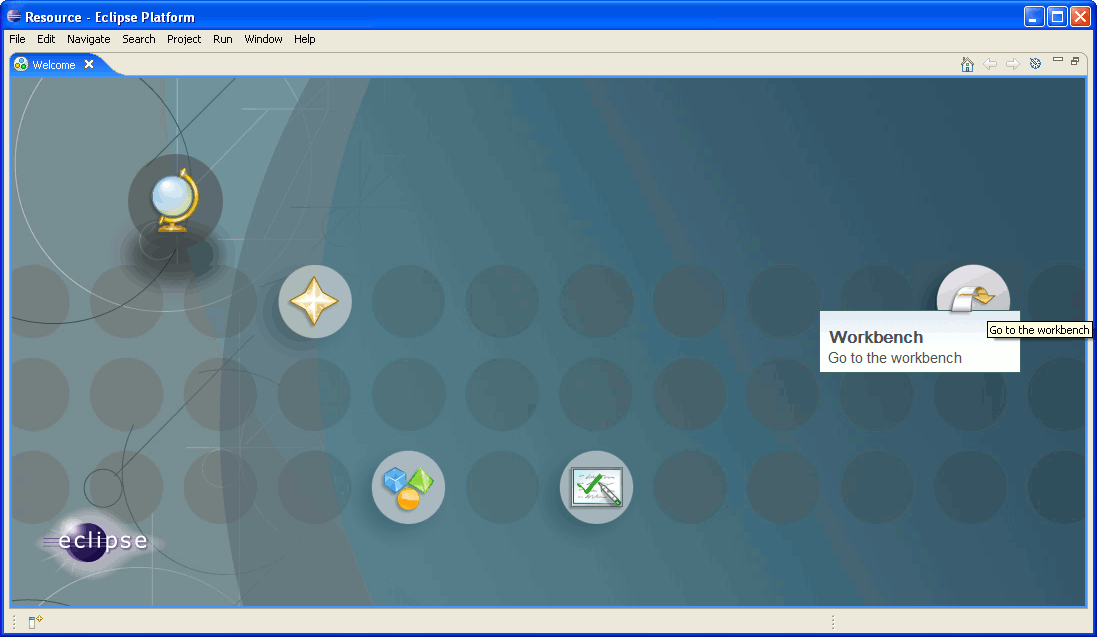
\includegraphics[
  width=12cm, bb=0 0 1097 637]{images/welcome.png}\end{center}
\caption{The Eclipse Welcome screen.}
\label{fig:welcome}
\end{figure}

\item
Before being able to correctly build your application, you should set
the path to the AVR-Gcc compiler. For doing so, please go to the
``Preference'' menu, as shown in Figure \ref{fig:preferences-menu},
and find the ``RT-Druid/Oil/Avr5 Configurator'' form as depicted in
Figure \ref{fig:preferences-avr5}.  The first textbox, labeled
\const{Gcc path}, refers to the installation directory of the AVR-Gcc
compiler.  The second and third textboxes are useful if you are using
a development environment based on the Crossbow Mib5x0 board. In
particular, the second textbox, labeled \const{Uisp path}, refers to
the installation directory of the uisp programmer for Crossbow Mib5x0
board, and the third textbox, labeled \const{Serial port device},
refers to the COM serial port where the board is attached.

\begin{warning}
The install directories specified for the AVR-Gcc Compiler in the textboxes 
of Figure \ref{fig:preferences-avr5} does {\em not} include the \file{bin}
directory! 

That is, \file{c:\\WinAVR-20071221} is correct, wheras
\file{c:\\WinAVR-20071221\\bin} is not.
\end{warning}


\begin{figure}[htb]
\begin{center}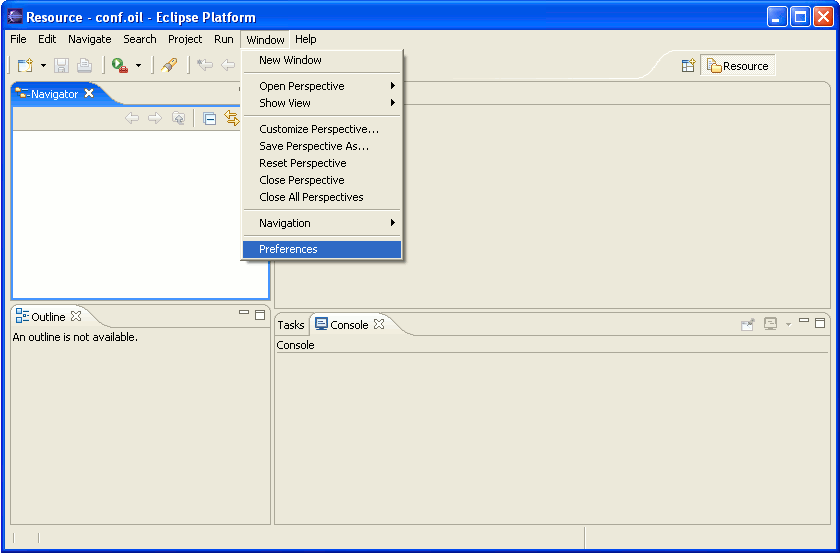
\includegraphics[
  width=8cm, bb=0 0 840 553]{images/preferences_menu.png}\end{center}
\caption{Go to the ``Preference'' menu.}
\label{fig:preferences-menu}
\end{figure}

\begin{figure}[htb]
\begin{center}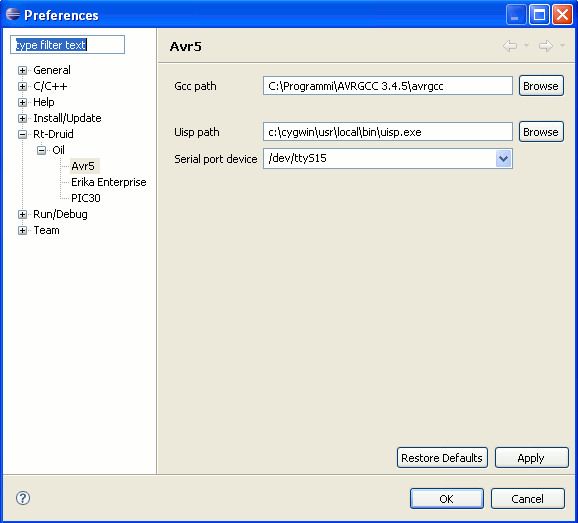
\includegraphics[
  width=8cm, bb=0 0 635 527]{images/preferences_avr5.png}\end{center}
\caption{Select paths for compiler and assembler.}
\label{fig:preferences-avr5}
\end{figure}

% ---

\item
  Before creating and building your application, please deselect the
  ``Build Automatically'' flag inside the ``Project'' menu, as shown
  in Figure \ref{fig:build-automatically}.
%
\begin{figure}[htb]
\begin{center}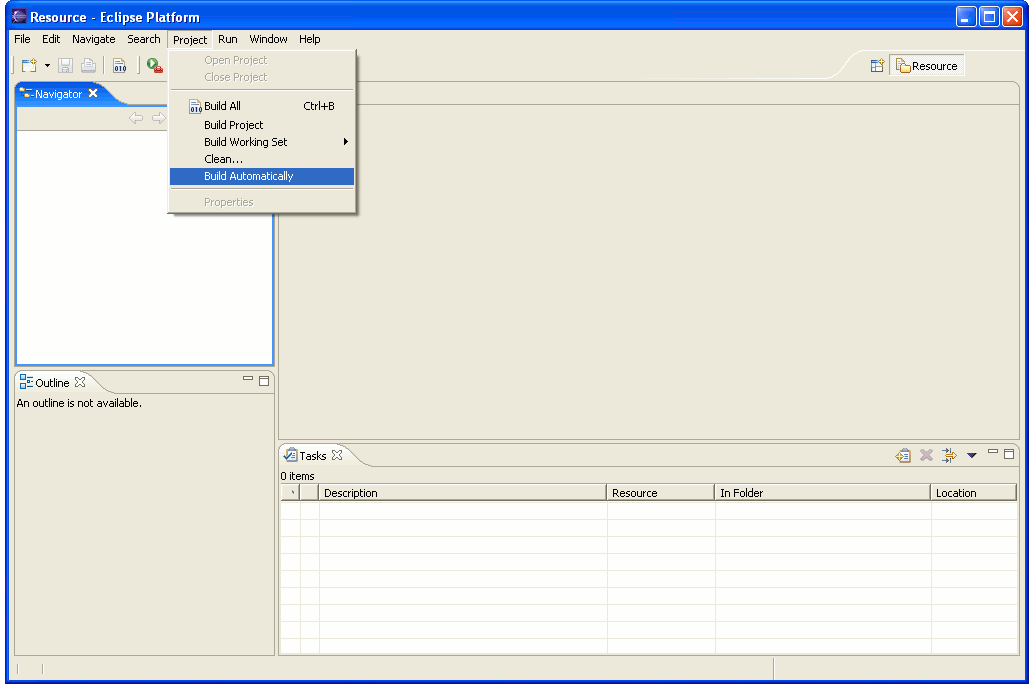
\includegraphics[
  width=8cm, bb=0 0 1029 684]{images/build_automatically.png}\end{center}
\caption{Deselect the ``Build Automatically'' flag in the ``Project'' menu.}
\label{fig:build-automatically}
\end{figure}

% ---

\end{enumerate}


\chapter{Compiling your first \ee\ demo for \avr5}

You are now ready to compile your first \ee\ demo. Please execute the
following steps:

\begin{enumerate}

\item
  Please select ``New Project'', then ``RT-Druid Oil and c/c++
  Project'' from the ``File menu'', as in Figure
  \ref{fig:new-project}.
%
\begin{figure}[htb]
\begin{center}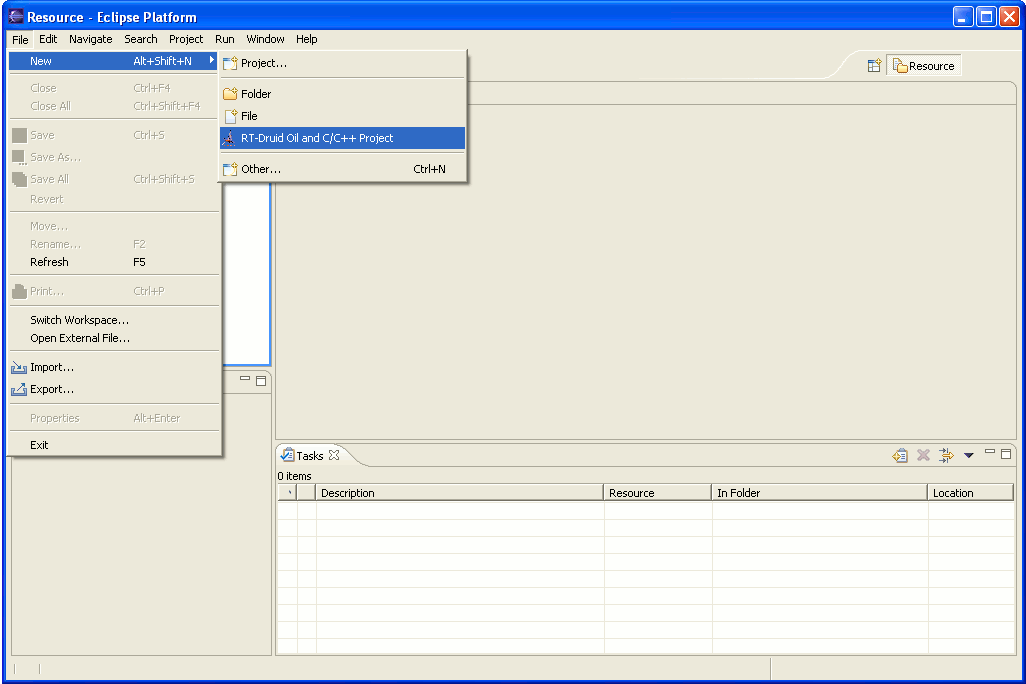
\includegraphics[
  width=12cm, bb=0 0 1026 684]{images/newproject.png}\end{center}
\caption{Select ``New project'' from the ``File'' menu.}
\label{fig:new-project}
\end{figure}

\item
  A Dialog box appear. Please select a template for the new project,
  as in Figure \ref{fig:new-project2}.
%
\begin{figure}[htb]
\begin{center}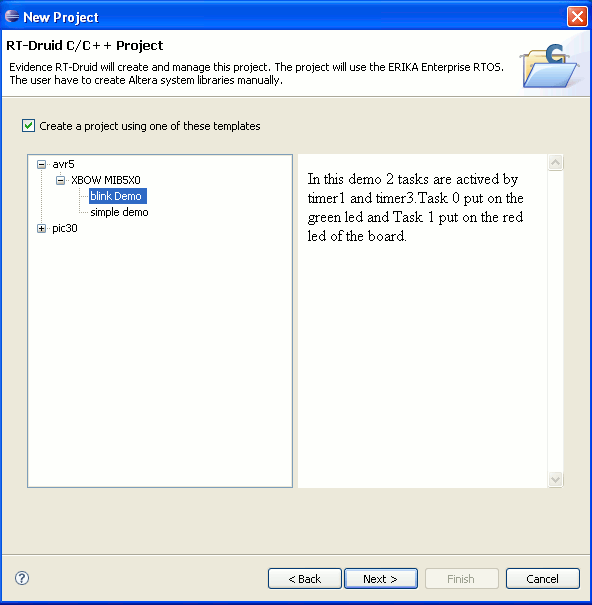
\includegraphics[
  width=8cm, bb=0 0 596 605]{images/newproject2.png}\end{center}
\caption{Select a template for your project.}
\label{fig:new-project2}
\end{figure}

\item
  Press ``Next''.

\item
  Insert the name of the new project. Please type \const{myProject}
  (you can choose other names of course). Please see Figure
  \ref{fig:projectname}. Press the ``Finish'' button.
%
\begin{figure}[htb]
\begin{center}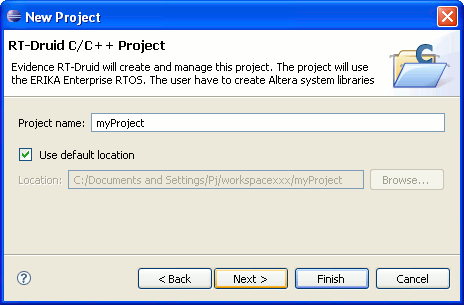
\includegraphics[
  width=8cm, bb=0 0 464 305]{images/projectname.png}\end{center}
\caption{Type a name for the new project.}
\label{fig:projectname}
\end{figure}

\item
  We are now ready to build the demo. Right click on the project name
  in the Eclipse navigation bar, and choose ``Build
  Project''\footnote{``Build Project'' only appears if the ``Build
  Automatically'' flag is not selected in the ``Project'' menu.} (see
  Figure \ref{fig:build-project}).
%
\begin{figure}[htb]
\begin{center}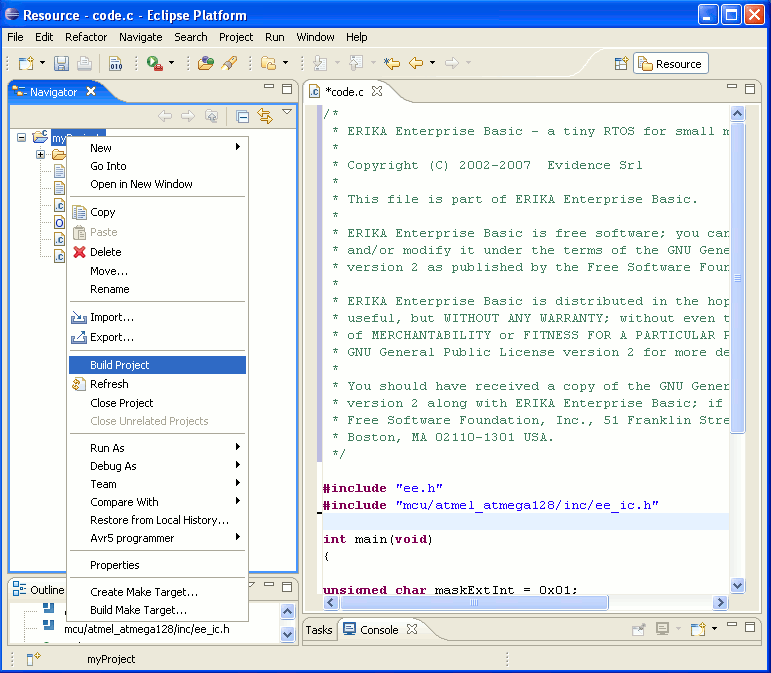
\includegraphics[
  width=10cm, bb=0 0 1024 684]{images/buil_project.png}\end{center}
\caption{We are now able to build the project.}
\label{fig:build-project}
\end{figure}

\item
  Then, the compilation process starts as depicted in Figure
  \ref{fig:compiling}. Please note the message that appears when the
  compilation is successfull.
%
\begin{figure}[htb]
\begin{center}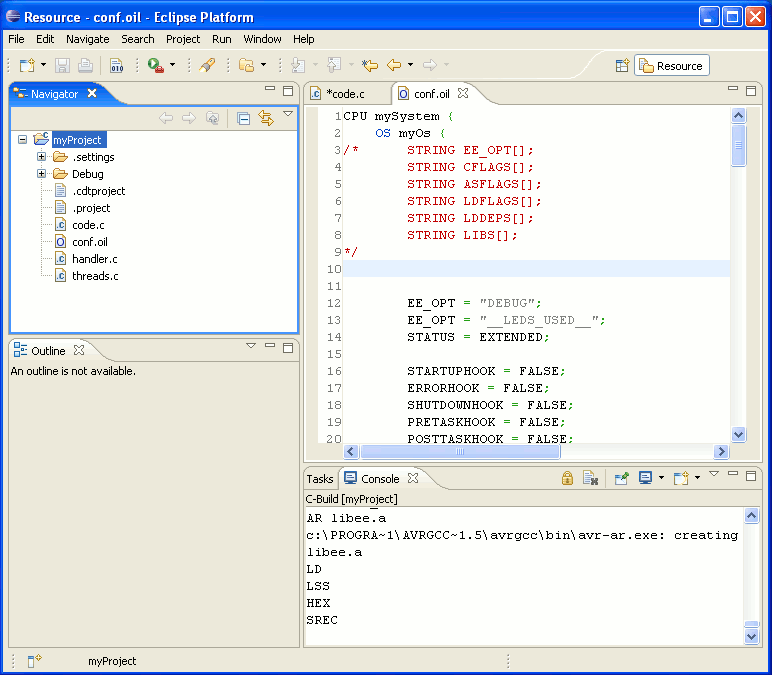
\includegraphics[
  width=10cm, bb=0 0 1097 637]{images/compiling.png}\end{center}
\caption{The compilation process.}
\label{fig:compiling}
\end{figure}

\begin{note}
  If the error depicted in Figure \ref{fig:mymake_cygwin_error} appears (meaning
  that \file{mymake_cygwin.bat} is unable to find a file), then please
  follow the instructions at the last point of Chapter
  \ref{cha:installing}.
\end{note}
%
\begin{figure}[htb]
\begin{center}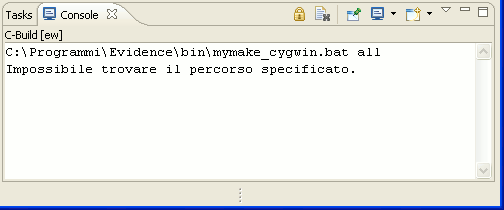
\includegraphics[
  width=10cm, bb=0 0 504 210]{images/mymake_cygwin_error.png}\end{center}
\caption{An error that shows up on some Windows machines. Please check 
the \file{mymake_cygwin.bat} file as explained in the last 
point of Chapter \ref{cha:installing}.}
\label{fig:mymake_cygwin_error}
\end{figure}

\item At the end of the compiling process you will be able to find a
  file named \file{avr.elf} and a file named \file{avr.srec} inside the 
  \file{Debug} directory inside the project, as shown in Figure
  \ref{fig:elf-file} and in the figure \ref{fig:srec-file}.

\begin{figure}[htb]
\begin{center}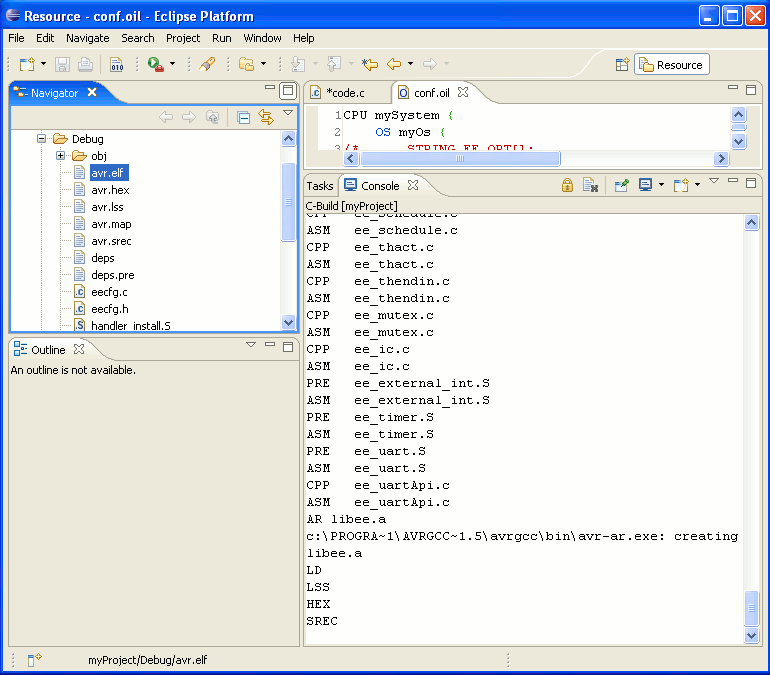
\includegraphics[
  width=10cm, bb=0 0 770 675]{images/elf_file.png}\end{center}
\caption{The output file is ready to be programmed on the target board.}
\label{fig:elf-file}
\end{figure}


\begin{figure}[htb]
\begin{center}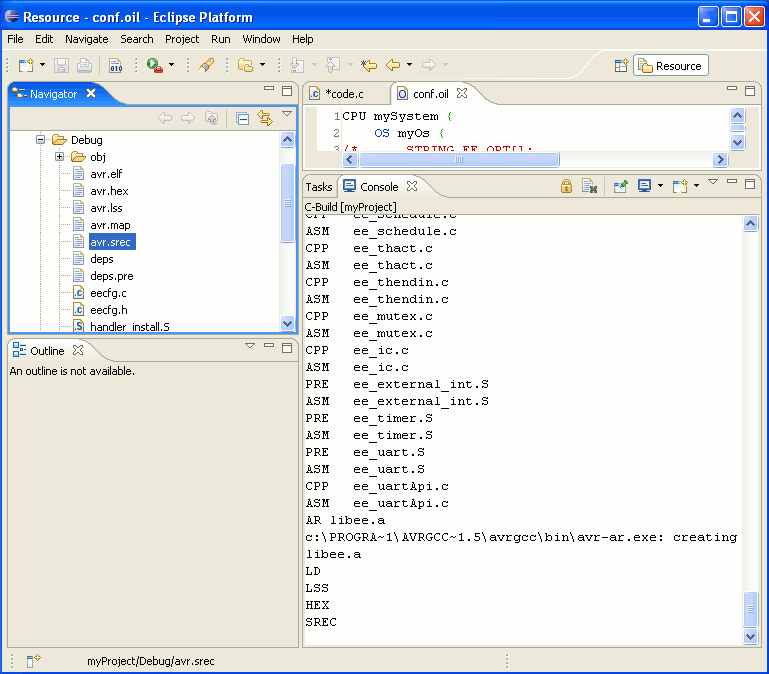
\includegraphics[
  width=10cm, bb=0 0 769 674]{images/srec_file.png}\end{center}
\caption{The output file is ready to be programmed on the target board.}
\label{fig:srec-file}
\end{figure}


\item
  You can now program the device using avr5 programmer as shown in Figure
  \ref{fig:progr-dev1} and in Figure \ref{fig:progr-dev2}.
  Please remember that you have to connect ISP6PIN plug of the STK500
  with the SPROG plug of the STK501 through 6-wires cable.
\end{enumerate}

\begin{figure}[htb]
\begin{center}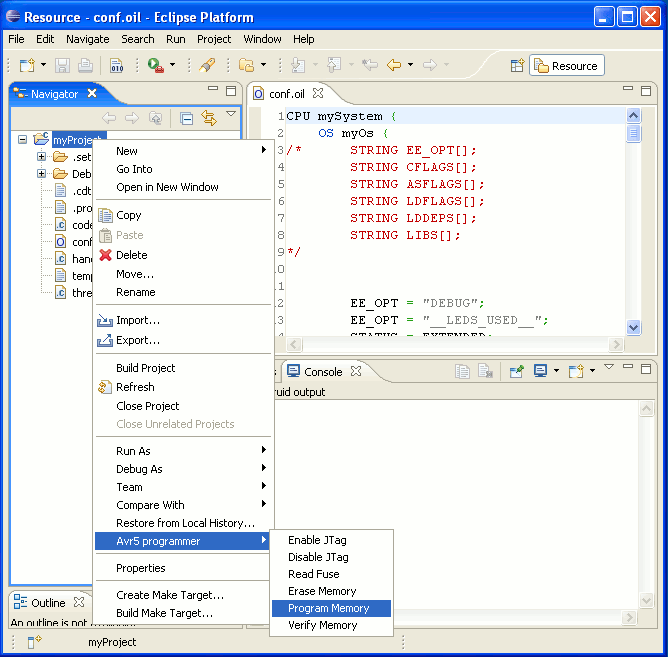
\includegraphics[
  width=12cm, bb=0 0 668 657]{images/program_device1.png}\end{center}
\caption{Program the Flash memory of the device.}
\label{fig:progr-dev1}
\end{figure}


\begin{figure}[htb]
\begin{center}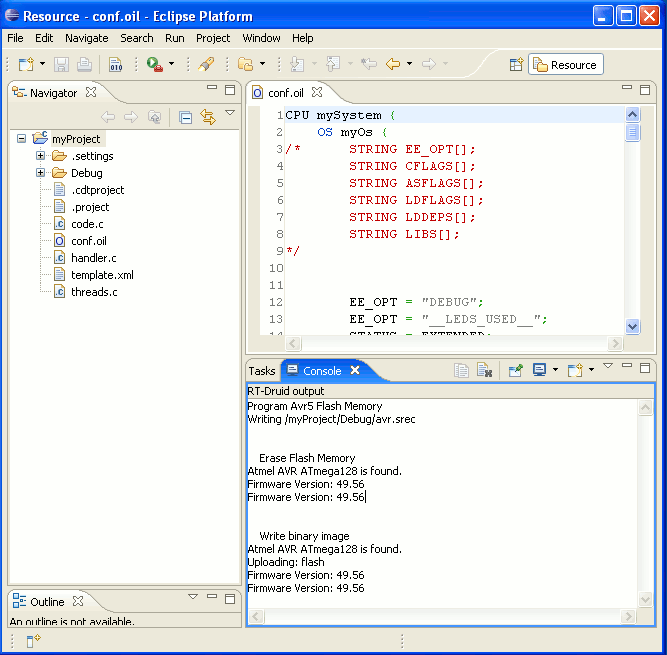
\includegraphics[
  width=12cm, bb=0 0 667 655]{images/program_device2.png}\end{center}
\caption{Program the Flash memory process.}
\label{fig:progr-dev2}
\end{figure}
